% filepath: /home/kluo/Documents/Repos/mathphy/homework/2026/hw3_sol.tex
% Solutions to Homework 3 — Math Physics Methods (数学物理方法)

\PassOptionsToPackage{quiet}{xeCJK}
\documentclass[11pt]{article}

\usepackage[margin=1in]{geometry}
\usepackage{amsmath,amsthm,amssymb,mathtools, graphicx, multicol, array}
\usepackage{ctex}
\usepackage{fancyhdr}
\usepackage{fontspec}
\usepackage{fourier-orns}
\usepackage{tikz}
\usetikzlibrary{decorations.markings,arrows.meta}

\newcommand{\N}{\mathbb{N}}
\newcommand{\Z}{\mathbb{Z}}
\newcommand{\R}{\mathbb{R}}
\newcommand{\C}{\mathbb{C}}

\theoremstyle{remark}
\newtheorem{problem}{}
\theoremstyle{definition}
\newtheorem{solution}{解}

\renewcommand{\headrule}{%
\vspace{-8pt}\hrulefill
\raisebox{-2.0pt}{\quad\decofourleft\decotwo\decofourright\quad}\hrulefill}

\setlength{\headheight}{15.11996pt}
\setlength{\topmargin}{-3.11996pt}

\newcommand{\duedate}{\zhdate{2026/10/13}}
\pagestyle{fancy}

\fancyhead{}
\fancyhead[L]{数学物理方法}
\zhnumsetup{style={Traditional,Financial}}
\fancyhead[R]{课后习题叁 \quad 参考解答}

\fancyfoot{}
\fancyfoot[C]{\thepage}
\fancyfoot[L]{截止日期\duedate}
\fancyfoot[R]{任课教师:罗凯}

\begin{document}
\renewcommand{\labelenumi}{(\arabic{enumi})}
\renewcommand{\labelenumii}{(\arabic{enumi}.\arabic{enumii})}

%==========================================================================
\begin{problem}
设 $\Psi(t, x)=e^{ \left(2 t x-t^2\right)}$, $t$是复变数, 试证:
\[
\left.\frac{\partial^n \Psi(t, x)}{\partial t^n}\right|_{t=0}=(-1)^n e^{x^2} \frac{d^n}{d x^n} e^{-x^2}.
\]
提示: 对回路积分进行积分变数的代换 $\xi=z-x$.
\end{problem}

\begin{solution}
$\Psi(t,x)=e^{(2tx-t^{2})}=e^{x^{2}}e^{-(x-t)^{2}}$.
令 $x$ 为参数，对 $t$ 利用柯西积分公式有
\[
\frac{\partial^{n}\Psi(t,x)}{\partial t^{n}}
=\Psi^{(n)}(t,x)
=\frac{n!}{2\pi\imath}\oint_{l}
\frac{e^{x^{2}}e^{-(x-\xi)^{2}}}{(\xi-t)^{n+1}}\,\mathrm{d}\xi.
\]
让 $\xi=x-z$，则 $\mathrm{d}\xi=-\mathrm{d}z$，$x-\xi=z$，
\begin{align*}
\Psi^{(n)}(t,x)
&=\frac{n!}{2\pi\imath}\oint_{l}
\frac{e^{x^{2}}e^{-z^{2}}}{(x-t-z)^{n+1}}(-\mathrm{d}z) \\
&=\frac{n!}{2\pi\imath}\oint_{l}
\frac{(-1)^{n}e^{x^{2}}e^{-z^{2}}}{\bigl[z-(x-t)\bigr]^{n+1}}\,\mathrm{d}z.
\end{align*}
令 $t=0$，
\begin{align*}
\left.\frac{\partial^{n}\Psi(t,x)}{\partial t^{n}}\right|_{t=0}
&=\frac{n!}{2\pi\imath}\oint_{l}
\frac{(-1)^{n}e^{x^{2}}e^{-z^{2}}}{(z-x)^{n+1}}\,\mathrm{d}z
=(-1)^{n}e^{x^{2}}\frac{\mathrm{d}^{n}}{\mathrm{d}x^{n}}e^{-x^{2}}.
\end{align*}
证毕。
\end{solution}

%==========================================================================
\begin{problem}
根据模最大原理,
求 $|\sin z|$ 在闭区域 $0 \leq \Re z \leq 2 \pi, 0 \leq \Im z \leq 2 \pi$ 中的最大值.
\end{problem}

\begin{solution}
模最大原理指解析函数 $f(z)$ 在边界上取模的极大值。此处边界有四条，对 $|\sin z|$ 在边界上的值分别讨论。

当 $x=0$，$0\leq y\leq 2\pi$ 时，
\[
|\sin z|=|\sin(\imath y)|=|\sinh y|,
\]
在 $y=2\pi$ 时取最大值 $|\sinh 2\pi|=\sinh 2\pi$。

当 $x=2\pi$，$0\leq y\leq 2\pi$ 时，由习题 2.1 的不等式得
\[
|\sin(x+\imath y)|\leq|\cosh y|\leq\cosh 2\pi,
\]
满足在边界上不超过 $\cosh 2\pi$。

当 $y=0$，$0\leq x\leq 2\pi$ 时，
\[
|\sin(x+\imath y)|=|\sin x|\leq 1.
\]

当 $y=2\pi$，$0\leq x\leq 2\pi$ 时，
\begin{align*}
|\sin(x+\imath y)|
&=\frac12\sqrt{\bigl(e^{\imath x-y}+e^{-\imath x+y}\bigr)
\bigl(e^{-\imath x-y}+e^{\imath x+y}\bigr)} \\
&=\frac12\sqrt{e^{2y}+e^{-2y}+2(\sin^{2}x-\cos^{2}x)}
=\frac12\sqrt{e^{4\pi}+e^{-4\pi}-2\cos 2x}.
\end{align*}
当 $x=\dfrac12\pi$ 或者 $\dfrac32\pi$ 时，$\cos 2x=-1$，所以有
\[
|\sin z|\leq\frac12\sqrt{e^{4\pi}+e^{-4\pi}+2}=\cosh 2\pi.
\]

综上最大值为 $\cosh 2\pi$。

\begin{center}
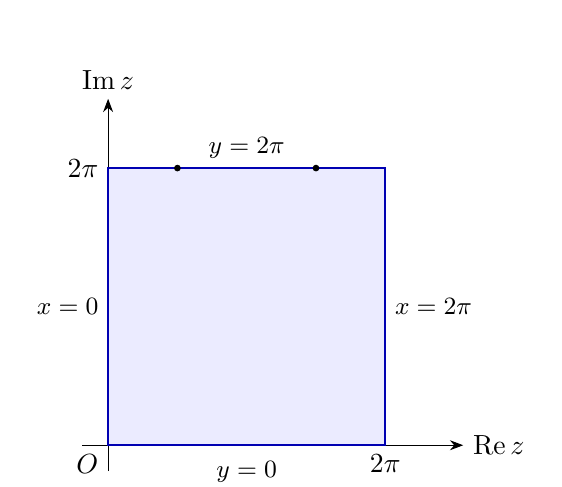
\begin{tikzpicture}[scale=0.55, >=Stealth]
  \draw[->] (-0.6,0) -- (8.2,0) node[right] {$\mathrm{Re}\,z$};
  \draw[->] (0,-0.6) -- (0,8.0) node[above] {$\mathrm{Im}\,z$};
  \fill[blue!8] (0,0) rectangle (6.4,6.4);
  \draw[thick, blue!70!black] (0,0) rectangle (6.4,6.4);
  \node[below] at (6.4,0) {$2\pi$};
  \node[left] at (0,6.4) {$2\pi$};
  \node[below left] at (0,0) {$O$};
  \fill (1.6,6.4) circle (2.2pt);
  \fill (4.8,6.4) circle (2.2pt);
  \node[above] at (3.2,6.4) {\small $y=2\pi$};
  \node[below] at (3.2,-0.15) {\small $y=0$};
  \node[left] at (0,3.2) {\small $x=0$};
  \node[right] at (6.4,3.2) {\small $x=2\pi$};
\end{tikzpicture}
\end{center}
\end{solution}

%==========================================================================
\begin{problem}
$f(z)$ 在全平面解析, 且 $|f(z)| \geq 1$, 用Liouville定理证明 $f(z)$ 为常数.
\\
提示:考虑$F(z) = \frac{1}{f(z)}$.
\end{problem}

\begin{solution}
$|f(z)|\geq 1$，则令 $F(z)=\dfrac{1}{f(z)}$。显然
\[
|F(z)|=\frac{1}{|f(z)|}\leq 1.
\]
因而 $F(z)$ 在全平面解析且有界，由刘维尔定理知 $F(z)$ 为常数，所以 $f(z)$ 为常数。
\end{solution}

%==========================================================================
\begin{problem}
设 $f(z)$ 在区域 $B$ 内解析, $C$ 为 $B$ 内任一简单闭曲线, 证明对于 $B$ 内,
但不在 $C$ 上的 任一点 $z$,
\[
\oint_C \frac{f^{\prime}(\xi)}{\xi-z} d \xi=\oint_C \frac{f(\xi)}{(\xi-z)^2} d \xi.
\]
\end{problem}

\begin{solution}
由题意，在区域 $B$ 内函数解析且 $z$ 在 $B$ 内、不在 $C$ 上。

若 $z$ 在 $C$ 内部，由柯西积分公式
\[
\oint_{C}\frac{f'(\xi)}{\xi-z}\,\mathrm{d}\xi=2\pi\imath\, f'(z),\qquad
\oint_{C}\frac{f(\xi)}{(\xi-z)^{2}}\,\mathrm{d}\xi=2\pi\imath\, f'(z),
\]
故两端相等。

若 $z$ 在 $C$ 外部，则两被积函数在 $C$ 所围区域内均解析，由柯西定理两端都等于 $0$，仍相等。

证毕。
\end{solution}

%==========================================================================
\begin{problem}
计算:
\begin{itemize}
  \item
  (i) $\int_{|z|=1} \frac{d z}{z}$;
  (ii) $\int_{|z|=1} \frac{d z}{|z|}$;
  (iii) $\int_{|z|=1} \frac{|d z|}{z}$;
  (iv) $\int_{|z|=1}\left|\frac{d z}{z}\right|$ .

  \item  $\oint_C \frac{\sin \frac{\pi z}{4}}{z^2-1} d z, C$ 分别为

  (i) $|z|=\frac{1}{2}$,
  (ii) $|z-1|=1$,
  (iii) $|z|=3$.

\end{itemize}
\end{problem}

\begin{solution}
\textbf{(1)}
令 $z=e^{\imath\theta}$，$\mathrm{d}z=\imath e^{\imath\theta}\,\mathrm{d}\theta$。
一般地
\[
\mathrm{d}z=e^{\imath\theta}\,\mathrm{d}r+\imath r e^{\imath\theta}\,\mathrm{d}\theta,\qquad
|\mathrm{d}z|=\sqrt{\mathrm{d}r^{2}+(r\mathrm{d}\theta)^{2}}.
\]
在 $|z|=1$ 上 $r=1$，$\mathrm{d}r=0$，故 $|\mathrm{d}z|=\mathrm{d}\theta$。

(i) 由于积分路径内部包含奇点 $z=0$，所以
\[
\int_{|z|=1}\frac{\mathrm{d}z}{z}=2\pi\imath.
\]

(ii)
\[
\int_{|z|=1}\frac{\mathrm{d}z}{|z|}
=\int_{0}^{2\pi}\frac{e^{\imath\theta}}{1}\imath\,\mathrm{d}\theta
=\imath\int_{0}^{2\pi}e^{\imath\theta}\,\mathrm{d}\theta=0.
\]

(iii)
\[
\int_{|z|=1}\frac{|\mathrm{d}z|}{z}
=\int_{0}^{2\pi}\frac{\mathrm{d}\theta}{e^{\imath\theta}}
=\int_{0}^{2\pi}e^{-\imath\theta}\,\mathrm{d}\theta=0.
\]

(iv)
\[
\int_{|z|=1}\left|\frac{\mathrm{d}z}{z}\right|
=\int_{0}^{2\pi}\left|\frac{\imath e^{\imath\theta}\,\mathrm{d}\theta}{e^{\imath\theta}}\right|
=\int_{0}^{2\pi}\mathrm{d}\theta=2\pi.
\]

\medskip
\textbf{(2)}
被积函数的奇点为 $z=\pm 1$。

(i) 路径不包含奇点 $z=1$、$z=-1$，因而被积函数解析，积分为 $0$，即
\[
\oint_{C}\frac{\sin\dfrac{\pi z}{4}}{z^{2}-1}\,\mathrm{d}z=0.
\]

(ii) 路径仅包含 $z=1$ 的奇点，
\begin{align*}
\oint_{C}\frac{\sin\dfrac{\pi z}{4}}{z^{2}-1}\,\mathrm{d}z
&=\oint_{C}\frac{1}{z-1}\cdot\frac{\sin\dfrac{\pi z}{4}}{2(z+1)}\,\mathrm{d}z
=2\pi\imath\cdot\frac12\sin\frac{\pi}{4}
=\frac{\sqrt2}{2}\pi\imath.
\end{align*}

(iii) 路径包含 $z=\pm 1$ 两个奇点，
\[
\oint_{C}\frac{\sin\dfrac{\pi z}{4}}{z^{2}-1}\,\mathrm{d}z
=2\pi\imath\cdot\frac12\sin\frac{\pi}{4}
-2\pi\imath\cdot\frac12\sin\Bigl(-\frac{\pi}{4}\Bigr)
=\sqrt2\,\pi\imath.
\]

\begin{center}
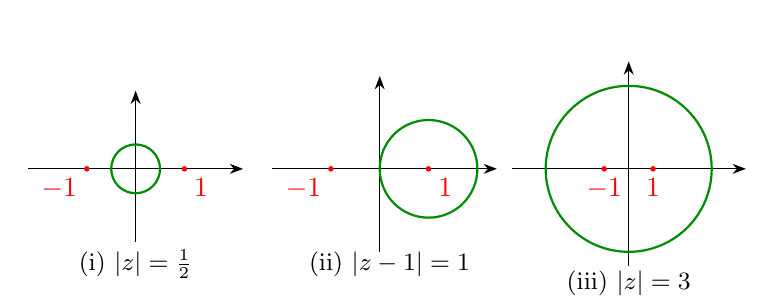
\begin{tikzpicture}[scale=0.62, >=Stealth]
  \begin{scope}
    \draw[->] (-2.2,0) -- (2.2,0);
    \draw[->] (0,-1.5) -- (0,1.6);
    \draw[green!55!black, thick] (0,0) circle[radius=0.5];
    \fill[red] (1,0) circle (1.6pt) node[below right] {$1$};
    \fill[red] (-1,0) circle (1.6pt) node[below left] {$-1$};
    \node at (0,-1.95) {\small (i) $|z|=\frac12$};
  \end{scope}
  \begin{scope}[xshift=5.0cm]
    \draw[->] (-2.2,0) -- (2.4,0);
    \draw[->] (0,-1.7) -- (0,1.9);
    \draw[green!55!black, thick] (1,0) circle[radius=1];
    \fill[red] (1,0) circle (1.6pt) node[below right] {$1$};
    \fill[red] (-1,0) circle (1.6pt) node[below left] {$-1$};
    \node at (0.2,-1.95) {\small (ii) $|z-1|=1$};
  \end{scope}
  \begin{scope}[xshift=10.1cm]
    \draw[->] (-2.4,0) -- (2.4,0);
    \draw[->] (0,-2.0) -- (0,2.2);
    \draw[green!55!black, thick] (0,0) circle[radius=1.7];
    \fill[red] (0.5,0) circle (1.6pt) node[below] {$1$};
    \fill[red] (-0.5,0) circle (1.6pt) node[below] {$-1$};
    \node at (0,-2.35) {\small (iii) $|z|=3$};
  \end{scope}
\end{tikzpicture}
\end{center}
\end{solution}

%==========================================================================
\begin{problem}
判断下列级数的收敛性及绝对收敛性:
\begin{enumerate}
    \item $\sum \frac{i^n}{\ln n}$;
    \item $\sum \frac{i^n}{n}$;
    \item  交错调和级数(除此之外，求其值).
\end{enumerate}
\end{problem}

\begin{solution}
\textbf{(1)}
\[
\sum_{n=2}^{\infty}\frac{\imath^{n}}{\ln n}
=\sum_{k=1}^{\infty}\frac{(-1)^{k}}{\ln(2k)}
+\sum_{k=0}^{\infty}\frac{\imath(-1)^{k}}{\ln(2k+1)}.
\]
求和项均为交错级数，$\displaystyle\lim_{k\to\infty}\frac{1}{\ln(2k)}=0$ 且 $\dfrac{1}{\ln(2k)}$ 单调递减，由莱布尼茨判据可知，求和项均收敛。
又
\[
\sum\left|\frac{\imath^{n}}{\ln n}\right|
=\sum_{n=2}^{\infty}\frac{1}{\ln n}
>\sum_{n=2}^{\infty}\frac{1}{n},
\]
发散，因此该级数条件收敛。

\textbf{(2)}
同 (1) 可得，$\sum\dfrac{\imath^{n}}{n}$ 收敛，又 $\sum\left|\dfrac{\imath^{n}}{n}\right|=\sum\dfrac{1}{n}$ 发散，因此原级数条件收敛。

\textbf{(3)}
交错调和级数 $\displaystyle\sum_{n=1}^{\infty}\frac{(-1)^{n+1}}{n}$。
由莱布尼茨判据，级数收敛；又 $\sum\dfrac{1}{n}$ 发散，故条件收敛。
根据课堂上列出的 $\ln(1+x) = \sum_{k=1}^{\infty}(-1)^{k+1}\dfrac{x^k}{k}$，
令 $x=1$ 得
\[
\ln(1+1) = \sum_{k=1}^{\infty}(-1)^{k+1}\dfrac{1^k}{k}=\ln 2.
\]
\end{solution}

%==========================================================================
\begin{problem}
确定下列级数的收敛半径（或收敛区域):
\begin{enumerate}
    \item $\sum z^n$;
    \item $\sum \frac{1}{2^n n^n} z^n$;
    \item $\sum \frac{n !}{n^n} z^n$;
    \item $\sum n^{\ln{n}} z^n$;
    \item $\sum 2^n \sin \frac{z}{3^n}$;
    \item $\sum \frac{\ln \left(n^n\right)}{n !} z^n$.
\end{enumerate}
\end{problem}

\begin{solution}
\textbf{(1)}
$\displaystyle\lim_{n\to\infty}\frac{1}{1}=1$，收敛半径 $R=1$，收敛区域 $|z|<1$。

\textbf{(2)}
\begin{align*}
R=\lim_{n\to\infty}\frac{a_{n}}{a_{n+1}}
&=\lim_{n\to\infty}\frac{2^{n+1}(n+1)^{n+1}}{2^{n}n^{n}}
=\lim_{n\to\infty}2\Bigl(1+\frac1n\Bigr)^{n}(n+1)=\infty.
\end{align*}

\textbf{(3)}
\begin{align*}
R=\lim_{n\to\infty}\frac{n!/n^{n}}{(n+1)!/(n+1)^{n+1}}
&=\lim_{n\to\infty}\frac{1}{n+1}\Bigl(\frac{n+1}{n}\Bigr)^{n}(n+1)
=\lim_{n\to\infty}\Bigl(1+\frac1n\Bigr)^{n}=e.
\end{align*}

\textbf{(4)}
\[
\lim_{n\to\infty}\sqrt[n]{n^{\ln n}}
=\lim_{n\to\infty}n^{\ln n/n}
=\lim_{n\to\infty}e^{(\ln n)^{2}/n}.
\]
根据洛必达法则，
\[
\lim_{n\to\infty}\frac{(\ln n)^{2}}{n}
=\lim_{n\to\infty}\frac{2\ln n}{n}
=\lim_{n\to\infty}\frac{2}{n}=0
\quad\Longrightarrow\quad
\lim_{n\to\infty}n^{\ln n/n}=e^{0}=1,
\]
故 $R=1$。

\textbf{(5)}
\[
\lim_{n\to\infty}\left|
\frac{2^{n+1}\sin\dfrac{z}{3^{n+1}}}{2^{n}\sin\dfrac{z}{3^{n}}}
\right|
=\lim_{n\to\infty}\left|
\frac{2^{n+1}\dfrac{z}{3^{n+1}}}{2^{n}\dfrac{z}{3^{n}}}
\right|
=\frac23<1,
\]
即不论 $z$ 取何值，级数均收敛，所以收敛半径为无穷，收敛域为整个复平面。

\textbf{(6)}
令
\[
a_{n}=\frac{\ln(n^{n})}{n!}=\frac{n\ln n}{n!}=\frac{\ln n}{(n-1)!},
\]
\begin{align*}
R=\lim_{n\to\infty}\frac{a_{n}}{a_{n+1}}
&=\lim_{n\to\infty}\frac{\ln n}{\ln(n+1)}\cdot\frac{n!}{(n-1)!}
=\lim_{n\to\infty}n\frac{\ln n}{\ln(n+1)}=\infty.
\end{align*}
\end{solution}

\end{document}
